\documentclass[12pt]{article}
\usepackage{fullpage}
\usepackage{amsmath,amssymb}
\usepackage{graphicx}
\usepackage[sort&compress,numbers,round]{natbib}
\usepackage{titlesec} % adjust section heading style
\usepackage[nolists,nomarkers]{endfloat} % put floats at end
\usepackage{lscape}  % make pages landscape
% \usepackage{rotating}
\usepackage{longtable} % long, er, tables

\DeclareDelayedFloatFlavour*{longtable}{table}

\titleformat{\section}
  {\normalfont\bf\large}{\thesection}{1em}{}
\titleformat{\subsection}
  {\normalfont\large\slshape}{\thesection}{1em}{}
\titleformat{\subsubsection}
  {\normalfont\slshape}{\thesection}{1em}{}

\renewcommand{\P}{\mathbb{P}}
\newcommand{\E}{\mathbb{E}}
\DeclareMathOperator{\cov}{cov}
\DeclareMathOperator{\var}{var}

\bibliographystyle{unsrtnat}

\topmargin 0.0cm
\oddsidemargin 0.2cm
\textwidth 16cm 
\textheight 21cm
\footskip 1.0cm


% Bold the 'Figure #' in the caption and separate it with a period
% Captions will be left justified
\usepackage[labelfont=bf,labelsep=period,justification=raggedright]{caption}

% \usepackage{hyperref}
\newcommand{\url}[1]{\texttt{#1}}
\newcommand{\email}[1]{\texttt{#1}}
\newcommand{\href}[2]{#2 (\texttt{#1})}


\usepackage{times}


\begin{document}

\appendix
\renewcommand{\thefigure}{S\arabic{figure}}
\setcounter{figure}{0}
\renewcommand{\thetable}{S\arabic{table}}
\setcounter{table}{0}

%%%%%%%%%%%%%%%%

\scriptsize

% tmp <- read.csv("table-s2.csv", header=TRUE, sep=",")
% levels(tmp$species) <- tolower(gsub("_"," ",levels(tmp$species)))
% substr(levels(tmp$species),1,1) <- toupper(substr(levels(tmp$species),1,1) )
% bold.these <- c( "LACM_84071", "LACM_86004", "LACM_91779", "LACM_84254", "LACM_84252", "LACM_88951", "LACM_88987", "LACM_84072", "LACM_84251", "LACM_84267" )
% tmpfn <- function (x) { gsub("_", "\\_", ifelse( x %in% bold.these, paste("\\textbf{",x,"}"), x ), fixed=TRUE ) }
% tmptable <- xtable(tmp,digits=1)
%  sink("table-s2.tex")
%  print.xtable(tmptable,include.rownames=FALSE,sanitize.text.function=tmpfn)
%  sink(NULL)
\begin{longtable}{|p{1.95in}p{1.1in}p{.15in}p{.4in}p{.4in}p{.4in}p{.4in}p{.4in}|}
  \caption{ Individual level data from bone scans.  NA indicates absence of sample in museum collection.  Numbers presented for bones are centroid sizes.  Museum source indicated in specimen column (BMNH=British Museum of Natural History, CCSN=Cape Cod Stranding Network, LACM=Los Angeles County Natural History Museum, MAL=Marine Animal Life, MH=New England Aquarium, MJM=Michael J. Moore, UMA=University of Massachusetts Amherst, USNM=United States Natural History Museum (Smithsonian), UWBM=University of Washington Burke Museum).  Specimens in bold were scanned multiple times to assess technical replication (one juvenile not shown).  }\\
  \hline
 \textbf{species} & \textbf{specimen} & \textbf{sex} & \textbf{body length} & \textbf{pelvic left} & \textbf{pelvic right} & \textbf{rib left} & \textbf{rib right} \\ 
\hline
\endfirsthead
\multicolumn{8}{c}%
{\tablename\ \thetable\ -- \textit{Continued from previous page}} \\
\hline
 \textbf{species} & \textbf{specimen} & \textbf{sex} & \textbf{body length} & \textbf{pelvic left} & \textbf{pelvic right} & \textbf{rib left} & \textbf{rib right} \\ 
\hline
\endhead
\hline \multicolumn{8}{r}{\textit{Continued on next page}} \\
\endfoot
\hline
\endlastfoot
  \hline
Balaenoptera acutorostrata & MAL\_03-282 & F & 730.0 & 2299.8 & 2246.1 & NA & NA  \\ 
  Balaenoptera acutorostrata & MH\_03-621 & M & 700.0 & 1898.3 & 1868.0 & NA & NA  \\ 
  Balaenoptera musculus & BMNH\_1953-12.1.18 & F & 2350.0 & 3862.8 & 3771.2 & NA & NA  \\ 
  Balaenoptera musculus & BMNH\_1953-12.1.19 & M & 2360.0 & 3765.0 & NA & NA & NA  \\ 
  Balaenoptera physalus & UMA\_4820 & F & 2075.0 & 2376.7 & 2405.2 & NA & NA  \\ 
  Delphinus capensis & \textbf{ LACM\_84071 } & M & 209.0 & 860.0 & 858.7 & 1221.3 & 1264.7 \\ 
  Delphinus capensis & LACM\_84127 & M & 215.0 & 736.7 & 737.6 & 1222.2 & 1243.3 \\ 
  Delphinus capensis & LACM\_84163 & M & 226.0 & 796.7 & 808.0 & 1473.7 & 1458.9 \\ 
  Delphinus capensis & LACM\_84185 & M & 211.5 & 907.7 & 898.7 & 1276.7 & 1346.0 \\ 
  Delphinus capensis & LACM\_84220 & M & 212.0 & 851.6 & 870.7 & 1361.0 & 1347.5 \\ 
  Delphinus capensis & LACM\_84221 & M & 218.5 & 853.1 & 840.8 & 1418.8 & 1442.4 \\ 
  Delphinus capensis & LACM\_84233 & M & 223.5 & 963.6 & 943.7 & 1280.4 & 1302.6 \\ 
  Delphinus capensis & LACM\_84236 & F & 208.0 & 677.1 & 695.4 & 1210.3 & 1227.1 \\ 
  Delphinus capensis & LACM\_84239 & M & 208.5 & 670.5 & 657.6 & 1356.7 & 1357.9 \\ 
  Delphinus capensis & LACM\_84240 & M & 235.0 & 884.6 & 868.9 & 1420.8 & 1429.1 \\ 
  Delphinus capensis & LACM\_84241 & M & 232.9 & 892.4 & 937.8 & NA & NA  \\ 
  Delphinus capensis & LACM\_85995 & M & 210.0 & 896.8 & 894.2 & 1463.8 & 1429.0 \\ 
  Delphinus capensis & \textbf{ LACM\_86004 } & M & 233.0 & 853.4 & 892.7 & 1454.6 & 1450.5 \\ 
  Delphinus capensis & LACM\_88979 & M & 211.5 & 902.6 & 903.3 & 1293.9 & 1297.8 \\ 
  Delphinus capensis & LACM\_88999 & M & 214.0 & 730.3 & 735.1 & NA & NA  \\ 
  Delphinus capensis & LACM\_91307 & F & 207.0 & 915.7 & 906.7 & 1270.0 & 1271.4 \\ 
  Delphinus capensis & \textbf{ LACM\_91779 } & M & 234.0 & 854.5 & 860.3 & 1306.3 & 1289.7 \\ 
  Delphinus capensis & LACM\_91915 & M & 222.0 & 895.8 & 928.2 & 1345.6 & 1360.4 \\ 
  Delphinus capensis & LACM\_92071 & M & 227.0 & 939.3 & 947.4 & 1454.0 & 1518.5 \\ 
  Delphinus capensis & LACM\_92077 & M & 222.5 & 987.2 & 1021.4 & 1342.3 & 1433.3 \\ 
  Delphinus capensis & LACM\_95668 & M & 218.0 & NA & NA & 1271.4 & 1241.8 \\ 
  Delphinus capensis & LACM\_96366 & M & 217.5 & 860.1 & 825.2 & 1382.1 & 1351.8 \\ 
  Delphinus capensis & LACM\_97203 & M & 219.0 & NA & 653.3 & NA & NA  \\ 
  Delphinus capensis & LACM\_97204 & M & 224.0 & 807.2 & 838.9 & NA & NA  \\ 
  Delphinus capensis & LACM\_97429 & M & 232.0 & 987.3 & 956.3 & 1477.3 & 1506.3 \\ 
  Delphinus capensis & LACM\_97478 & M & 212.0 & 851.8 & 855.3 & 1460.5 & 1455.7 \\ 
  Delphinus delphis & \textbf{ LACM\_84254 } & M & 229.0 & 938.2 & 915.4 & 1395.5 & 1391.7 \\ 
  Delphinus delphis & USNM\_504107 & M & 209.0 & 989.3 & 996.2 & 1379.4 & 706.2 \\ 
  Delphinus delphis & USNM\_572632 & M & 223.0 & 870.3 & 852.7 & NA & 1357.1 \\ 
  Delphinus delphis & USNM\_572775 & M & 203.0 & 1097.2 & 1097.6 & 1361.3 & 1434.8 \\ 
  Delphinus delphis & USNM\_572776 & M & 228.0 & 983.2 & 991.2 & 1388.7 & 1388.4 \\ 
  Delphinus delphis & USNM\_572777 & M & 216.0 & 922.4 & 924.3 & 1305.4 & 1426.2 \\ 
  Delphinus delphis & USNM\_572859 & F & 207.0 & 820.8 & 839.3 & 1357.6 & 1347.0 \\ 
  Delphinus delphis & USNM\_572871 & M & 229.0 & NA & 1051.0 & 1311.3 & 1283.7 \\ 
  Delphinus delphis & USNM\_572980 & M & 225.0 & 1028.1 & 1016.2 & 1449.1 & 1387.5 \\ 
  Eschrichtius robustus & UWBM\_35430 & M & 1293.0 & 4557.0 & NA & NA & NA  \\ 
  Eubalaena glacialis & MJM\_070110 & M & 1370.0 & 4305.6 & 4471.8 & NA & NA  \\ 
  Eubalaena glacialis & UMA\_4920 & F & 1370.0 & 3432.7 & 3395.9 & NA & NA  \\ 
  Feresa attenuata & \textbf{ LACM\_84252 } & M & 214.0 & 1082.9 & 1090.3 & 1334.6 & 1345.3 \\ 
  Feresa attenuata & USNM\_550389 & M & 212.0 & 1049.2 & 1049.8 & NA & 1351.9 \\ 
  Feresa attenuata & USNM\_571268 & M & 230.0 & 993.6 & 1001.5 & 1517.2 & 1522.4 \\ 
  Globicephala melas & CCSN\_04-141 & F & 460.0 & 1306.4 & 1175.8 & NA & NA  \\ 
  Grampus griseus & LACM\_72546 & M & 360.7 & 1208.7 & 1192.7 & 2347.2 & 2380.0 \\ 
  Grampus griseus & USNM\_504126 & M & 298.0 & 1125.2 & 1107.5 & 1976.2 & 2007.2 \\ 
  Grampus griseus & USNM\_550391 & M & 286.0 & 988.5 & 1020.2 & 1926.1 & 1922.7 \\ 
  Inia geoffrensis & LACM\_19590 & M & 240.0 & 988.5 & 1013.9 & 1462.4 & 1493.0 \\ 
  Inia geoffrensis & LACM\_27074 & M & 228.0 & 940.7 & 898.0 & 1567.9 & 1641.4 \\ 
  Lagenorhynchus acutus & USNM\_504154 & F & 234.5 & 860.0 & 853.9 & 1580.8 & 1562.2 \\ 
  Lagenorhynchus acutus & USNM\_550995 & M & 253.0 & 959.1 & 995.1 & 1618.7 & 1610.3 \\ 
  Lagenorhynchus acutus & USNM\_571327 & M & 253.0 & 843.3 & 907.9 & 1578.4 & 1588.3 \\ 
  Lagenorhynchus acutus & USNM\_571390 & M & 242.0 & 968.0 & 978.3 & 1550.5 & 1566.8 \\ 
  Lagenorhynchus obliquidens & LACM\_84284 & M & 220.0 & 902.3 & 967.9 & 1572.0 & 1517.1 \\ 
  Lagenorhynchus obliquidens & \textbf{ LACM\_88951 } & M & 192.0 & 885.5 & 856.2 & 1528.5 & 1465.4 \\ 
  Lagenorhynchus obliquidens & \textbf{ LACM\_88987 } & M & 207.0 & 771.8 & 778.0 & 1475.7 & 1454.0 \\ 
  Lagenorhynchus obliquidens & LACM\_92062 & M & 194.0 & 733.2 & 757.2 & 1386.8 & 1417.4 \\ 
  Lagenorhynchus obliquidens & LACM\_95514 & F & 223.0 & 765.2 & 717.1 & 1588.5 & 1686.0 \\ 
  Lissodelphis borealis & LACM\_72455 & M & 264.4 & 999.8 & 1010.6 & 1343.2 & 1358.5 \\ 
  Lissodelphis borealis & LACM\_95689 & M & 217.8 & 974.3 & 987.5 & 1161.6 & 1245.6 \\ 
  Lissodelphis borealis & USNM\_484929 & M & 265.3 & 1128.5 & 1139.6 & 1489.9 & 1536.7 \\ 
  Mesoplodon carlhubbsi & USNM\_504128 & F & 532.0 & 1007.1 & 1043.3 & 3119.4 & 3124.1 \\ 
  Peponocephala electra & LACM\_54090 & F & 231.0 & 1008.1 & 974.6 & 1611.4 & 1635.9 \\ 
  Phocoena phocoena & LACM\_72591 & M & 148.0 & 1063.1 & 1058.3 & NA & NA  \\ 
  Phocoena phocoena & \textbf{ LACM\_84072 } & M & 154.0 & 1018.1 & 995.4 & 1491.8 & 1475.3 \\ 
  Phocoena phocoena & LACM\_84073 & F & 173.0 & 829.5 & 872.4 & 1403.8 & 1414.0 \\ 
  Phocoena phocoena & LACM\_84076 & F & 178.0 & 945.3 & 997.7 & 1409.8 & 1415.6 \\ 
  Phocoena phocoena & LACM\_84086 & F & 164.5 & 880.5 & 877.0 & 1319.0 & 1317.5 \\ 
  Phocoena phocoena & USNM\_504302 & F & 165.0 & 834.4 & 917.4 & 1275.9 & 1279.1 \\ 
  Phocoena phocoena & USNM\_550312 & F & 158.0 & 897.4 & 879.9 & 1334.4 & 1362.6 \\ 
  Phocoena phocoena & USNM\_571709 & M & 160.2 & 1155.7 & 1159.7 & 1409.4 & 1352.6 \\ 
  Phocoena phocoena & USNM\_571723 & M & 146.1 & 1094.4 & 1086.9 & 1125.8 & 1152.4 \\ 
  Phocoena phocoena & USNM\_572629 & F & 163.0 & 718.3 & 775.9 & 1361.7 & 1374.8 \\ 
  Phocoena phocoena & USNM\_572785 & M & 151.5 & 1108.1 & 1110.9 & 1299.1 & 1328.9 \\ 
  Phocoenoides dalli & LACM\_54420 & M & 203.0 & 793.8 & 846.7 & 1679.6 & 1600.2 \\ 
  Phocoenoides dalli & LACM\_54569 & F & 200.0 & 690.3 & 695.7 & 1748.3 & 1747.2 \\ 
  Phocoenoides dalli & LACM\_84048 & M & 213.0 & 590.0 & 575.1 & 1568.3 & 1510.1 \\ 
  Phocoenoides dalli & \textbf{ LACM\_84251 } & M & 225.0 & 686.9 & 733.8 & 1749.3 & 1753.2 \\ 
  Phocoenoides dalli & LACM\_96383 & M & 213.5 & 770.1 & 777.2 & 1556.0 & 1514.2 \\ 
  Phocoenoides dalli & LACM\_96487 & M & 210.0 & 557.9 & NA & NA & NA  \\ 
  Phocoenoides dalli & LACM\_97207 & M & 210.0 & 691.5 & 677.9 & NA &  NA \\ 
  Phocoenoides dalli & USNM\_396304 & M & 202.0 & 795.3 & 794.9 & 1567.3 & 1566.4 \\ 
  Pontoporia blainvillei & LACM\_47143 & M & 128.5 & 302.0 & 297.5 & 774.5 & 803.6 \\ 
  Pontoporia blainvillei & LACM\_54012 & F & 138.0 & 396.6 & 364.7 & 848.7 & 861.0 \\ 
  Pontoporia blainvillei & USNM\_501157 & F & 136.0 & 343.5 & 325.3 & 833.2 & 842.3 \\ 
  Pontoporia blainvillei & USNM\_501172 & M & 137.0 & NA & NA & 720.1 & 764.6 \\ 
  Pontoporia blainvillei & USNM\_501176 & F & 142.0 & 340.0 & 343.2 & 798.8 & 846.6 \\ 
  Pontoporia blainvillei & USNM\_501179 & M & 142.0 & 407.2 & 428.4 & 797.5 & 834.9 \\ 
  Pontoporia blainvillei & USNM\_501183 & F & 145.0 & 285.2 & 295.8 & 828.4 & 883.0 \\ 
  Pontoporia blainvillei & USNM\_501186 & F & 143.0 & 355.9 & 288.3 & 793.3 & 794.0 \\ 
  Pontoporia blainvillei & USNM\_504920 & F & 155.0 & 490.4 & 443.4 & 880.8 & 911.0 \\ 
  Pseudorca crassidens & LACM\_84047 & M & 480.0 & 1379.1 & 1362.4 & 2352.0 & 2415.8 \\ 
  Stenella attenuata & LACM\_54043 & M & 195.0 & 651.2 & 628.4 & 1144.1 & 1155.2 \\ 
  Stenella attenuata & LACM\_95489 & F & 191.9 & 572.8 & 545.6 & 1157.5 & 1170.1 \\ 
  Stenella attenuata & USNM\_395277 & F & 175.0 & 646.1 & 643.2 & NA & NA  \\ 
  Stenella attenuata & USNM\_395390 & M & 218.0 & 722.1 & 707.3 & 1112.3 & 1128.2 \\ 
  Stenella attenuata & USNM\_395465 & M & 200.0 & 759.0 & 712.4 & 1116.3 & NA  \\ 
  Stenella coeruleoalba & USNM\_504350 & M & 231.0 & 737.4 & 740.6 & 1473.1 & 1459.4 \\ 
  Stenella coeruleoalba & USNM\_504773 & M & 221.7 & 669.9 & 662.8 & 1564.6 & 1532.2 \\ 
  Stenella frontalis & USNM\_504758 & M & 201.0 & 742.5 & 736.4 & 1434.6 & 1462.4 \\ 
  Stenella longirostris & LACM\_72437 & M & 175.4 & 541.2 & 579.8 & 1009.1 & 975.9 \\ 
  Stenella longirostris & LACM\_72438 & M & 177.5 & 651.7 & 664.0 & 1179.8 & 1198.3 \\ 
  Stenella longirostris & USNM\_395599 & M & 173.0 & 692.4 & 702.7 & 1161.8 & 1157.9 \\ 
  Steno bredanensis & USNM\_504467 & M & 235.0 & 737.0 & 761.0 & NA & 1672.7 \\ 
  Steno bredanensis & USNM\_504468 & M & 227.0 & 745.8 & 741.6 & NA & 1628.7 \\ 
  Steno bredanensis & USNM\_504494 & M & 233.0 & 748.6 & 818.3 & NA & 1393.5 \\ 
  Steno bredanensis & USNM\_550837 & M & 228.1 & 787.4 & 780.2 & 1538.6 & 1488.7 \\ 
  Tursiops aduncus & USNM\_258642 & M & 287.0 & 905.2 & 914.7 & 1900.4 & 1927.8 \\ 
  Tursiops truncatus & LACM\_84194 & M & 304.0 & 1108.3 & 1156.8 & 1827.2 & 1876.1 \\ 
  Tursiops truncatus & \textbf{ LACM\_84267 } & M & 305.0 & 865.6 & 868.1 & 1941.6 & 1838.3 \\ 
  Tursiops truncatus & LACM\_84271 & F & 285.0 & 663.1 & 616.9 & 1720.5 & 1704.1 \\ 
  Tursiops truncatus & LACM\_92072 & M & 288.0 & 746.3 & 717.5 & 1768.1 & 1785.2 \\ 
  Tursiops truncatus & LACM\_95828 & M & 293.0 & 959.0 & 939.2 & NA & NA  \\ 
  Tursiops truncatus & LACM\_97405 & F & 277.0 & 842.1 & 955.1 & 1705.4 & 1709.0 \\ 
  Tursiops truncatus & LACM\_97489 & F & 298.0 & 1083.8 & 1045.8 & 1817.7 & 1914.5 \\ 
  Tursiops truncatus & USNM\_396165 & M & 303.0 & 796.7 & 876.0 & 1911.5 & NA  \\ 
  Tursiops truncatus & USNM\_504726 & M & 298.0 & 1068.1 & 1094.0 & 2014.3 & 1940.9 \\ 
  Tursiops truncatus & USNM\_504879 & M & 284.0 & 1000.5 & 1000.5 & NA & 1874.6 \\ 
  Tursiops truncatus & USNM\_550401 & M & 267.5 & 1073.7 & 1046.9 & 1701.2 & 1697.5 \\ 
  Tursiops truncatus & USNM\_550422 & M & 279.0 & 1155.2 & 1150.8 & 1812.2 & 1782.7 \\ 
  Tursiops truncatus & USNM\_550919 & F & 283.0 & 953.6 & 966.2 & 1833.0 & 1810.8 \\ 
  Tursiops truncatus & USNM\_571051 & M & 277.0 & 999.0 & 1024.7 & 1766.0 & 1763.1 \\ 
  Tursiops truncatus & USNM\_571086 & M & 273.0 & 1078.9 & 1030.9 & 1644.9 & 1723.9 \\ 
  Tursiops truncatus & USNM\_571388 & F & 285.0 & 790.6 & 830.5 & 1491.6 & 1509.5 \\ 
  Tursiops truncatus & USNM\_571521 & M & 271.0 & 659.5 & 669.7 & 1399.0 & 1396.5 \\ 
  Tursiops truncatus & USNM\_572949 & M & 265.0 & 1166.0 & 1105.4 & 1697.1 & 1644.7 \\ 
  Tursiops truncatus & USNM\_593406 & M & 279.0 & 1167.8 & 1172.6 & 1736.8 & 1770.7 \\ 
  Ziphius cavirostris & USNM\_A20971 & F & 589.0 & 854.0 & 828.4 & 3676.2 & 3580.3 \\ 
  Ziphius cavirostris & USNM\_A49599 & M & 564.0 & 978.7 & 1067.3 & 4095.2 & 3972.7 \\ 
   \hline
\end{longtable}

%%%%%%%%%%%%%%%%

\small

% tmp <- read.table("table-s1.csv",header=TRUE,sep='\t')
% tmp$references <- paste("cite{", tolower( sapply( lapply( strsplit(gsub("[{}]","",tmp$references),";"), function (z) gsub(", *", "", gsub( " #.*", "", z ) ) ), paste, collapse="," ) ), "}", sep='' )
% tmptab <- xtable(tmp)
% print(tmp,sanitize.text.function=identity)
% latex table generated in R 3.0.2 by xtable 1.7-1 package
% Sat Oct 19 20:51:35 2013
\begin{longtable}{|p{2.1in}p{0.5in}p{1.0in}p{1.0in}p{1.5in}|}
  \caption{Morphological data gathered from literature for sexually mature males.}\\
  \hline
  \textbf{species} & \textbf{max body length} & \textbf{maximum body mass} & \textbf{maximum testes mass} & \textbf{references} \\ 
\hline
\endfirsthead
\multicolumn{5}{c}%
{\tablename\ \thetable\ -- \textit{Continued from previous page}} \\
\hline
  \textbf{species} & \textbf{max body length} & \textbf{max body mass} & \textbf{max testes mass} & \textbf{references} \\ 
\hline
\endhead
\hline \multicolumn{5}{r}{\textit{Continued on next page}} \\
\endfoot
\hline
\endlastfoot
  \hline
          Balaena mysticetus  &         1800 &    90000000  &     163000.0   &                                    \citet{burns1993}   \\
  Balaenoptera acutorostrata  &          880 &     9200000  &       8800.0   &                                  \citet{tomilin1967} \\
       Balaenoptera borealis  &         1520 &          NA  &      16400.0   &                                    \citet{perry1999} \\
          Balaenoptera edeni  &         1500 &    40000000  &      20000.0   &                                  \citet{tomilin1967} \\
       Balaenoptera musculus  &         2700 &   150000000  &      70000.0   &                                  \citet{tomilin1967} \\
       Balaenoptera physalus  &         2400 &    90000000  &      58300.0   &                                \citet{jefferson2008} \\
           Caperea marginata  &          550 &          NA  &       1900.0   &                                    \citet{baker1985} \\
 Cephalorhynchus commersonii  &          174 &       86000  &        930.0   &                                  \citet{goodall1994} \\
          Delphinus capensis  &          250 &      235000  &       3785.0   &                       \citet{jefferson2008,ross1979} \\
           Delphinus delphis  &          270 &      200000  &       5000.0   &                                \citet{jefferson2008} \\
       Eschrichtius robustus  &         1500 &    45000000  &      67500.0   &                                  \citet{tomilin1967} \\
         Eubalaena japonica   &         1700 &    90000000  &     972000.0   &                                     \citet{best2001} \\
            Feresa attenuata  &          264 &      225000  &        754.0   &                                \citet{jefferson2008} \\
  Globicephala macrorhynchus  &          700 &     3600000  &       7000.0   &                                \citet{jefferson2008} \\
          Globicephala melas  &          670 &     2320000  &      12300.0   &                  \citet{jefferson2008,desportes1993} \\
             Grampus griseus  &          383 &      500000  &      10600.0   &                     \citet{jefferson2008,perrin1984} \\
            Inia geoffrensis  &          255 &      207000  &       1600.0   &                       \citet{jefferson2008,best1989} \\
             Kogia breviceps  &          425 &      417000  &      10000.0   &   \citet{bloodworth2008,caldwell1971,tomilin1967,ruiz1993} \\
                  Kogia sima  &          270 &      280000  &       2618.0   &                                     \citet{ross1979} \\
       Lagenorhynchus acutus  &          280 &      235000  &        740.0   &                                \citet{jefferson2008} \\
  Lagenorhynchus obliquidens  &          250 &      200000  &       1118.0   &                                 \citet{harrison1972} \\
       Lissodelphis borealis  &          307 &      115000  &       1410.0   &                                 \citet{harrison1972} \\
      Megaptera novaeangliae  &         1700 &    40000000  &       4000.0   &                                \citet{jefferson2008} \\
       Mesoplodon carlhubbsi  &          540 &     1500000  &        510.0   &                       \citet{jefferson2008,mead1982} \\
           Monodon monoceros  &          480 &     1600000  &           NA   &                                \citet{jefferson2008} \\
    Neophocaena phocaenoides  &          200 &       55000  &        863.0   &                                   \citet{kasuya1999} \\
                Orcinus orca  &          975 &    10000000  &      23100.0   &                       \citet{jefferson2008,ross1979} \\
       Peponocephala electra  &          278 &      275000  &       4500.0   &                                \citet{jefferson2008} \\
           Phocoena phocoena  &          180 &       61000  &       3515.0   &                                     \citet{read1999} \\
          Phocoenoides dalli  &          240 &      200000  &        560.0   &                                \citet{jefferson2008} \\
            Physeter catodon  &         1800 &    57000000  &      12000.0   &                                \citet{jefferson2008} \\
      Pontoporia blainvillei  &          160 &       50000  &         10.8   &                                \citet{jefferson2008} \\
        Pseudorca crassidens  &          600 &     2000000  &      14800.0   &                                \citet{jefferson2008} \\
          Stenella attenuata  &          257 &      120000  &       2896.0   &                       \citet{jefferson2008,hohn1985} \\
       Stenella coeruleoalba  &          256 &      160000  &        500.0   &                                 \citet{miyazaki1977} \\
          Stenella frontalis  &          230 &      140000  &       1210.0   &                                   \citet{perrin1994} \\
       Stenella longirostris  &          235 &       82000  &       2708.0   &                                \citet{jefferson2008} \\
           Steno bredanensis  &          265 &      160000  &       2660.0   &                                 \citet{miyazaki1994} \\
            Tursiops aduncus  &          270 &      230000  &           NA   &                                    \citet{wells1999} \\
          Tursiops truncatus  &          381 &      650000  &       1966.0   &                                   \citet{perrin1984} \\
         Ziphius cavirostris  &          700 &     3000000  &       4200.0   &                                    \citet{omura1955} \\
  \hline
\end{longtable}

\normalfont


\noindent
\begin{center}
\textbf{Supplementary Materials for}\\
Cetacean pelvic bones are targets of sexual selection

Dines, J. P.*, E. Ot\'arola-Castillo, P. Ralph, J. Alas, T. Daley, A. D. Smith, M. D. Dean*\\
*Correspondence: \email{jdines$@$nhm.org}, \email{matthew.dean$@$usc.edu}
\end{center}

\noindent
\textbf{This file includes:}
\begin{enumerate}
    \item Materials and Methods
    \item Figures S1--S7
    \item Tables S1--S12
    \item Full Reference List
\end{enumerate}

\pagebreak

% \nocite{adams2012,baker1985,best2001,best1989,bloodworth2008,bookstein1997,brownell1986,burns1993,caldwell1971,desportes1993,goodall1994,harrison1972,hohn1985,jefferson2008,kasuya1999,mcgowen2009,mead1982,mitteroecker2009,miyazaki1977,miyazaki1994,omura1955,pagel1999,paradis2004,perrin1994,perrin1984,perry1999,read1999,ross1979,ruiz1993,tomilin1967,wells1999,zelditch2004}
\nocite{uhen2010,perrin2013,schulte1918,pabst1998,meek1918,mate2005,brownell1986,fitzpatrick2012,ramm2005,firman2008,kenagy1986,moller1989,harcourt1981,moller1991,stockley1997,gage1994,hosken2001,suppmat,danilewicz2004,mcgowen2009,revell2009,heyning1994,rohlf1990,slice2007,adams2012,bookstein1997,bookstein1996,mitteroecker2009,gunz2005,mcardle2001,vanbree1973,andersen1992,perrin1975,eberhard1985,arnqvist1998,hosken2004,ramm2007}

\section*{Materials and Methods}
All original data and analytical code have been deposited in the Dryad Digital Repository (\url{http://dx.doi.org/10.5061/dryad.[NNNN]}). 

\subsection*{Re-analysis of penis length data}
\citet{brownell1986} published data on penis length, body length, and testis size from 10 baleen whale species.  We reanalyzed those data in a phylogenetically controlled, generalized least-squares model, using the gls procedure in the R package nlme, with a correlation structure that accounts for phylogenetic relatedness \citep{pagel1999}, using the corPagel procedure in the R package ape \citep{paradis2004}.  We first calculated the phylogenetic residuals of log penis length and log testis weight each regressed onto the log of body length.  Under the same phylogenetically controlled generalized least-squares model, residual penis length was significantly correlated to residual testis weight (P<10-10, Fig. S1).  A generalized correlation coefficient was then calculated. 

\subsection*{Scanning bones and identifying landmarks}
All bones were scanned with a NextEngine 3-dimensional Laser Scanner, returning tens of thousands of $x,y,z$ points per bone.  A pipeline was developed to sub-sample 962 evenly spaced and ordered points.  The pipeline is graphically illustrated for pelvic bones (Fig. S2) and ribs (Fig. S3) separately.  All original laser scans and the associated code for imposing landmarks has been made available on the Dryad Digital Repository (\url{http://dx.doi.org/10.5061/dryad.[NNNN]}). 

\subsection*{Technical replication}
We quantified technical replication by randomly choosing 41 bones (21 pelvic bones, 20 ribs) to scan more than once.  One bone was scanned 11 times, the rest scanned twice, each time removing the bone from the scanner and reloading it.  The median coefficient of variation (unbiased standard deviation/mean) for centroid size was 0.0094 for pelvic bones, 0.0090 for ribs.  The median coefficient of variation for shape variation was .0194 for pelvic bones, .0342 for ribs.  In sum, digitizing bones with the NextEngine Laser Scanner and our analytical pipeline (Fig. S2 and S3) produced highly repeatable results.  

\subsection*{Phylogenetic modeling}
We built a customized phylogenetic model to test for correlated evolution of testes size and bone centroid size.  The sample-specific morphological data (Table S1-S2) were placed on a cetacean phylogeny constructed from 45 nuclear loci, transposons, and mitochondrial genomes \citep{mcgowen2009}.  The logarithms of all values were then modeled as evolving on the tree as correlated Gaussian traits, accounting for intraspecific and intraindividual variation and missing data.  Priors were placed on the 16 covariances of this model (including separate parameters for within-species variation), and the posterior distribution was evaluated using Markov chain Monte Carlo.  All associated code for running these analyses have been made available on the Dryad Digital Repository (\url{http://dx.doi.org/10.5061/dryad.[NNNN]}).
To test whether bone shape evolution was correlated with differences in testis size, we first identified 9 independent species pairs for which both ribs and pelvic bones were sampled from adult males.  We tested whether the average pairwise distance between bones of each species was correlated with the absolute value of the difference in testis residuals calculated as above.  All code for running these analyses have been made available on the Dryad Digital Repository (\url{http://dx.doi.org/10.5061/dryad.[NNNN]}).
 



%%%%%%%%%%%
\subsection*{Correlated trait evolution}

It is clear that cetacean testes size, rib bone size, and pelvic bone size
should evolve in a correlated manner over evolutionary time
due to their common correlation with total body size 
(which varies considerably from dolphins to baleen whales);
to discover whether pelvic bone and testes size changes are correlated
after accounting for body size changes
requires a joint model of their evolution along the phylogeny.

The general framework we used to analyze these data is similar to those used in \citet{revell2009phylogenetic} and \citet{harmon2008geiger},
modified to account for within-species variation,
missing data,
and measurement of different variables at the species and/or individual level.
We do not account for uncertainty in the phylogeny,
as suggested by \citet{huelsenbeck2003detecting},
since it is unclear how much we should let body length and bone size influence branch lengths,
and we do not think that uncertainty in phylogeny will be a significant confounding factor.

Specifically, we have the following information about a number of individual whales:
species, sex, body length,
and the sizes of the right and left pelvic and anterior-most pair of vertebral rib bones
(although some of the measurements are missing).
Furthermore, for each species, we have
adult male body length and
breeding male testes volume.

There are three levels of variation:
between species (i.e.\ changes across branches in the phylogeny),
between individuals in a species,
and between left and right pairs of bones in each individual.
These can be visually put into a common framework by 
labeling the species tips of the phylogeny as the ``species mean'',
attaching additional edges to each species for each observed individual of that species (``individual edges'').
Trait differences are then written as the sum over trait changes along intervening edges.
For instance, the difference between a particular left rib size and the species mean rib size
is the sum of the difference between the rib size and that individual's mean rib sizes 
and the difference between that individual's mean and the species mean rib size.
Differences between two samples from different species include terms for both individuals' deviations from their species means,
as well as changes in species mean trait values along each edge of the phylogeny that separates the two species.
The species-level observation of testes size is treated as direct observation of the species mean;
since we do not observe testes size in inviduals, omitting modeling the observation error should not affect the analysis.

The inclusion of within-individual variation suggests attaching two additional branches of a third type
to each individual's tip;
however, it simplifies the analysis to instead treat left rib and right rib size 
as separate traits that evolve on the phylogeny,
but to assume that their evolution is perfectly correlated except on edges corresponding to intraspecific variation
(and similarly for left and right pelvic size).

% \begin{figure}
% XXX figure of (a) cetacean phylogeny we use; and (b) schematic with indiv \& sample edges XXX
% \end{figure}

We then model the observed set of trait values as resulting from correlated changes across this ramified phylogeny,
with different sets of parameters for each of the three types of edges.
Concretely, we take logarithms of all quantitative traits,
and model their evolution as a correlated Brownian motion.
We write these four traits as
\begin{align}
    L &= \log \text{(body length)}, \\
    T &= \log \text{(testes volume)}, \\
    P^R &= \log \text{( right pelvic centroid size )}, \\
    P^L &= \log \text{( left pelvic centroid size )}, \\
    R^R &= \log \text{( right rib centroid size )}, \\
    R^L &= \log \text{( left rib centroid size )},
\end{align}
and now need to specify our parameterization of the covariance across each type of branch.

\subsubsection*{Species differences}

First consider the difference of two species means across an internal (species) edge of length $t$ in the phylogeny.
Writing $X_0=(L_0,T_0,R^R_0,R^L_0,P^R_0,P^L_0)$ for the mean trait values of the ancestor,
and $X_t=(L_t,T_t,R^R_t,R^L_t,P^R_t,P^L_t)$ for the mean trait values of the descendant,
our model is that $X_t = X_0 + \sqrt{t} A Z$, with $Z$ independent standard Gaussians and $A_t$ the matrix given here:
\begin{align} \label{eqn:species_matrix}
\begin{bmatrix}
    L_t \\ T_t \\ R^R_t \\ R^L_t \\ P^R_t \\ P^L_t 
\end{bmatrix}
=
\begin{bmatrix}
    L_0 \\ T_0 \\ R^R_0 \\ R^L_0 \\ P^R_0 \\ P^L_0 
\end{bmatrix}
+
\sqrt{t}
\begin{bmatrix}
    \sigma_L &  0  & 0  & 0  \\
    \delta_T   &  \beta_T   & 0  &   0 \\
    \delta_R   &  \beta_R   & \sigma_R   &   0 \\
    \delta_R   &  \beta_R   & \sigma_R   &   0 \\
    \delta_P   &  \beta_P   & 0  &   \sigma_P  \\
    \delta_P   &  \beta_P   & 0  &   \sigma_P  
\end{bmatrix}
\begin{bmatrix}
    Z_1 \\ Z_2 \\ Z_3 \\ Z_4
\end{bmatrix}
\end{align}
In this parameterization, the covariance matrix of the trait differences $(X_t - X_0)$ is $\Sigma_t = A_t A_t^T$;
effectively, we are parameterizing the covariance matrix through its Cholesky decomposition,
subject to the constraint that left and right bone size changes are perfectly correlated.
A direct parameterization of $\Sigma_t$ is difficult to optimize over due to the complex constraits imposed by
the condition that $\Sigma_t$ be nonnegative definate;
the constraints on $A_t$ are only that the diagonal elements are positive \citep{pourahmadi1999joint}.

%
\subsubsection*{Individual variation}

We use a similar parameterization for within-species and within-individual variation.
If the species mean trait values are $X_S = (L_S,T_S,R^R_S,R^L_S,P^R_S,P^L_S)$ 
and the trait values of an individual are $X_I = (L_I,T_I,R^R_I,R^L_I,P^R_I,P^L_I)$,
then we write $X_I = X_S + B W$, again with $W$ independent standard Gaussians,
and $B$ parameterized by
\begin{align} \label{eqn:sample_matrix}
\begin{bmatrix}
    L_I \\
    T_I \\
    R^R_I \\
    R^L_I \\
    P^R_I \\
    P^L_I
\end{bmatrix}
=
\begin{bmatrix}
    L_S \\
    T_S \\
    R^R_S \\
    R^L_S \\
    P^R_S \\
    P^L_S
\end{bmatrix}
+
\begin{bmatrix}
    \zeta_L  &   0 & 0  & 0  & 0 \\
    - & - & - & - & - \\
    \eta_R  & \zeta_R   &  \omega_R  & 0 & 0 \\ 
    \eta_R  & \zeta_R   & - \omega_R & 0 & 0\\ 
    \eta_P  & 0 & 0 &  \zeta_P  & \omega_P  \\ 
    \eta_P  & 0 & 0 &  \zeta_P  & - \omega_P
\end{bmatrix}
\begin{bmatrix}
W_1 \\W_2 \\W_3 \\W_4 \\ W_5  \\ 
\end{bmatrix}
\end{align}
Here the row of $B$ corresponding to testes size is omitted because we do not observe testes size in individuals;
this will not enter the analysis.
In this form, 
$\zeta_R^2$ parameterizes the within-species variance of individual mean rib sizes,
and $\omega_R^2$ parameterizes the variance of rib sizes within an individual.

Note that this effectly assumes that within-species variation is of the same magnitude for each species,
and furthermore no substructure within each species.
If these are not good assumptions, one could add individual-level random effects (for instance);
but we did not see evidence that this was necessary.


%%
\subsubsection*{Mean-centering the data}

Above we have given a complete model for correlated trait evolution along a phylogeny,
including within-species variation,
given the trait values at the root.
It is usual in phylogenetics to compute the independent contrasts -- 
effectively, performing a linear transformation of the tip values that (a) renders them independent of the root value
and (b) results in jointly independent values.
The second property is merely a computational convenience, while the first property is essential.
This would be straightforward in this model if the species-level matrices $A$ and the individual-level matrices $B$ were jointly diagonalizable 
\citep[as in][]{revell2009phylogenetic}.

Fortunately, if we subtract any unbiased estimate of the root value, we obtain values that do not depend on the root value.
To see this, let $X_{ik}$ denote the matrix of trait values at the tips, with rows corresponding to individuals, 
and let $M_{ik}$ be a matrix whose columns sum to 1, so that 
$\bar X_k = \sum_i M_{ik} X_{ik}$ is an estimate of the $k^\mathrm{th}$ trait at the root.
Also write $dX_e$ for the vector of trait differences across edge $e$ in the tree,
and $X_\rho$ for the trait values at the root,
so that $X_i = X_\rho + \sum_{e \in \rho \to i} dX_e$,
where $\{e \in \rho \to i\}$ are the edges in the path from the root to tip $i$.
Then the centered observations $\widetilde X_{ik} := X_{ik} = \bar X_k$ do not depend on $X_\rho$:
if we assign weight $M_{ek}$ to each edge $e$ proportional to the weights that $M$ assigns to tips below it,
i.e.\ $M_{ek} = \sum_{i : e \in \rho \to i} M_{ik}$, then
\begin{equation} \label{eqn:mean_centering}
  \widetilde X_{ik} = \sum_{e \in \rho \to i} dX_{ek} - \sum_e M_{ek} dX_{ek} ,
\end{equation}
which does not depend on the trait values at the root.

For the weights $M$ that estimate the trait values at the root,
we use the ``phylogenetic mean'' \citep{felsenstein1973maximumlikelihood},
calculated independently for each trait,
using fairly short values for the branch lengths of the individual edges estimated from within-species variances,
as that should be fairly close to the minimum-variance estimator of the root values.
Note that the columns of $M$ are \emph{not} identical,
due to the irregular pattern of missing data.

\subsubsection*{Likelihood computation}

So far, we have given the covariance matrices for differences in trait values across each edge ($dX_e$ in the notation above),
have assumed that these values are independent for each edge,
and we now need to convert this to a covariance matrix for the data we do actually observe,
mean-centered as described above.
Since the mean-centered data are by assumption centered Gaussian, 
this is all we need to compute the likelihood of the data, given the covariance parameters in \eqref{eqn:species_matrix} and \eqref{eqn:sample_matrix}.

Suppose that $U$ is a $n$-dimensional Gaussian vector with covariance matrix $\Sigma$ (the edge differences $dX_e$ in some order),
and $V = Q U$ is a linear transformation of $U$ by the matrix $Q$ (the observed data),
then $V$ is also Gaussian, with covariance matrix $\widetilde \Sigma = Q \Sigma Q^T$.
Again, we have $\Sigma$ but would like $\widetilde \Sigma$.
Note above in equation \eqref{eqn:mean_centering} that the mean-centered data is a linear transformation of the differences across edges,
so that it is only a matter of bookkeeping to find the matrix $C$ corresponding to this transformation.
However, the matrix $C \Sigma C^T$ will be singular, since mean-centering reduces the number of degrees of freedom (here by four, as we subtract four trait means).
A simple computational way around this is to take $Q$ to be a projection matrix into the column space of $C$,
and to transform both the data and the covariance matrix by $Q$ as above.
Since weights $M$ assign zero influence to missing values in the data,
$Q$ will automatically omit such missing values: the columns of $Q$ corresponding to missing values will be zero.
(Another choice would to be to let $P$ be the matrix that drops one individual, and take $Q = PC$; 
but this is less numerically robust
and becomes trickier in the presence of missing data.)

Now that we have the covariance function, the computation is standard:
recalling that $Y$ is the transformed, mean-centered data and $\widetilde \Sigma(\theta)$ is the covariance matrix of $Y$,
which depends on the parameters $\theta$,
\begin{equation} \label{eqn:likelihood}
    \mathcal{L}(Y|\theta) = \frac{ 1 }{ \left( 2 \pi \det{\widetilde \Sigma(\theta)} \right)^{n/2} } \exp \left( - \frac{1}{2} Y^T {\widetilde \Sigma(\theta)} Y \right) .
\end{equation}
To compute this, we do the following:
\begin{enumerate}
    \item Compute the full covariance matrix $\Sigma(\theta)$ from the parameters $\theta$.
    \item Compute $\widetilde \Sigma(\theta) = Q \Sigma Q^T$ (note that $Q$ does not depend on the parameters).
    \item Compute $\det{\widetilde \Sigma(\theta)}$ and $Y^T {\widetilde \Sigma(\theta)} Y$ from the Cholesky decomposition of $\widetilde \Sigma(\theta)$ (found numerically).
\end{enumerate}
The first step is simplified by precomputation of appropriate matrices to place the parameters into the appropriate slots of $\Sigma$.


%%
\subsubsection*{Priors and Bayesian methods}

Now that we have an easily computible likelihood function,
we put priors on each of the parameters,
and estimate the posterior distribution of the parameters given the data
by a standard random-walk Markov chain Monte Carlo  (MCMC)
(as implemented in the \texttt{mcmc} package \citep{geyer2013mcmc} in R, \citet{R}).

% # return positive log-likelihood times posterior
% #  parameters are: sigmaL, betaT, betaP, sigmaR, sigmaP, zetaL, zetaR, omegaR, zetaP, omegaP, sigmaLdeltaT, sigmaLdeltaP, sigmaLdeltaR, zetaLdeltaP, zetaLdeltaR, 
% # priors are Gaussian with these SDs
% prior.means <- c(3,3,3,3,3,3,.1,.1,.1,.1,.1,1,1,1,.1,.1)
% # constrain these to be nonnegative:
% nonnegs <- c("sigmaL", "betaT", "sigmaR", "sigmaP", "zetaL", "zetaR", "omegaR", "zetaP", "omegaP" )
% nonneg.inds <- match( nonnegs, names(initpar) )
% stopifnot( length(prior.means) == length(initpar) )
% lud <- function (par) {
%     if (any(par[nonneg.inds]<=0)) { return( -Inf ) }
%     fullmat <- make.fullmat( par )[havedata,havedata]
%     submat <- ( ( crossprod( pmat, fullmat) %*% pmat ) )
%     fchol <- chol(submat)
%     return( (-1/2) * sum( (par / prior.means)^2 ) - sum( backsolve( fchol, datavec, transpose=TRUE )^2 )/2 - sum(log(diag(fchol))) )
% }

Roughly speaking, the parameters controlling variances are 
$\sigma_L$, $\beta_T$, $\sigma_R$, $\sigma_P$, $\zeta_L$, $\zeta_R$, $\omega_R$, $\zeta_P$, and $\omega_P$.
Those controlling covariances are $\delta_T$, $\delta_R$, $\delta_P$, $\beta_R$, $\beta_P$, $\eta_R$, and $\eta_P$.
We placed independent zero-mean Gaussian priors on all parameters, conditioning the variance parameters to be nonzero.
Based on examination of variability in various traits, we set
the prior standard deviations of $\sigma_L$, $\beta_T$, $\beta_P$, $\sigma_R$, $\sigma_P$, and $\zeta_L$ to 3,
the prior standard deviations of $\delta_T$, $\delta_R$, and $\delta_P$ to 1,
and the prior standard deviations of $\zeta_R$, $\omega_R$, $\zeta_P$, $\omega_P$, $\beta_R$, $\eta_R$, and $\eta_P$ to 0.1.


%%%%%
\subsubsection*{Proportion of changes explained by mating ecology}

It is of interest to estimate what proportion of changes in pelvic bone size are due to shifts in mating ecology,
relative to other causes, e.g.\ changes in species mean body length or random drift.
Under the model described above (equation \eqref{eqn:species_matrix}):
\begin{align}
   dP &= \delta_P dZ_1 + \beta_P dZ_2 + \sigma_P dZ_4 ,
 \end{align}
where each $dZ$ are independent white noise terms, each having the same variance.
$dZ_1$ corresponds to normalized changes in body length,
$dZ_2$ corresponds to normalized changes in testes size after accounting for changes in body length,
and $dZ_4$ is pelvic-specific noise.
Therefore, 
\begin{align}
  \frac{ \beta_P }{ \delta_P + \beta_P  + \sigma_P }
\end{align}
is a measure of the proportion of changes in pelvic bone size changes that are accounted for by changes in testes size.
There is an analogous measure for ribs.



%%%%%
\subsubsection*{Running the MCMC sampler}

To carefully check that our results were not affected by patterns of missing data,
we ran an MCMC sampler to estimate the posterior distribution of the above parameters
on three datasets:
\textbf{(a)} all bones from adult male cetaceans,
\textbf{(b)} all bones from adult female cetaceans,
and \textbf{(c)} all bones from adult male cetaceans for which we had data from both ribs and pelvic bones.
The dataset (c) is a subset of (a);
these differed primarily because the ribs of most baleen whales were too large to scan on available equipment,
so comparisons between ribs and pelvic bones in dataset (a) could potentially misleading.
As described below, results from (c) did not differ substantially from (a),
so we present the results of (a) in the main text.
Each dataset was run using the same pipeline, 
by simply setting the relevant observations to missing.

In each case, the MCMC sampler was run for a total of 500,000 iterations,
the first 20,000 of which were discarded as burn-in,
at which point it was apparent from trace plots that convergence had been reached.


\section*{Results}

Here we present additional results from the analysis of correlation trait evolution on the cetacean phylogeny described above.

\subsection*{Full dataset for males}

The summary statistics of the estimated posterior distributions 
for the parameters
are given in table~\ref{tab:posterior_distrns}.
Taking posterior mean values, we see that $0.07/(0.47+0.07+0.07)=0.11$ of the changes in pelvic bone size 
is derivable from shifts in testes size after removing the effects of length shifts,
an equal quantity is pelvic-specific noise,
and only $0.78$ comes from changes in body length.

% latex table generated in R 3.0.2 by xtable 1.7-1 package
% Wed Oct 16 16:35:12 2013
\begin{table}[ht]
    \footnotesize
\centering
\begin{tabular}{rrrrrrrrrrrrrrrrr}
  \hline
        &  $\sigma_L$  &  $\beta_T$  &  $\beta_P$  &  $\beta_R$  &  $\sigma_R$  &  $\sigma_P$  &  $\zeta_L$  &  $\zeta_R$   \\
\hline
5\%     &  0.11        &  0.38       &  0.03       &  -0.02      &  0.03        &  0.05        &  0.04       &  0.06        \\
25\%    &  0.14        &  0.44       &  0.05       &  -0.01      &  0.03        &  0.06        &  0.04       &  0.07        \\
mean    &  0.55        &  0.55       &  0.07       &  0.00       &  0.04        &  0.07        &  0.04       &  0.07        \\
75\%    &  0.51        &  0.61       &  0.08       &  0.01       &  0.05        &  0.07        &  0.05       &  0.07        \\
95\%    &  2.28        &  0.88       &  0.11       &  0.03       &  0.06        &  0.09        &  0.05       &  0.08        \\
   \hline
  \hline
        &    $\omega_R$  &  $\zeta_P$  &  $\omega_P$  &  $\delta_T$  &  $\delta_R$  &  $\delta_P$  &  $\eta_R$  &  $\eta_P$  \\
\hline
5\%     &    0.04        &  0.10       &  0.01        &  0.08        &  0.09        &  0.05        &  0.02      &  -0.00     \\
25\%    &    0.04        &  0.11       &  0.02        &  0.27        &  0.11        &  0.08        &  0.03      &  0.01      \\
mean    &    0.04        &  0.12       &  0.02        &  1.60        &  0.51        &  0.47        &  0.03      &  0.02      \\
75\%    &    0.04        &  0.13       &  0.02        &  3.29        &  0.43        &  0.54        &  0.04      &  0.02      \\
95\%    &    0.05        &  0.14       &  0.02        &  4.27        &  2.00        &  1.99        &  0.05      &  0.04      \\
   \hline
\end{tabular}
\caption{ \label{tab:posterior_distrns} Posterior means and quantiles of the parameters of the model presented in equations \eqref{eqn:species_matrix} and \eqref{eqn:sample_matrix}, estimated using only bones from adult males.  }
\end{table}

The correlation matrix for changes along a branch at the posterior mean parameter values is 
%  xtable( cov2cor(species.covmat)[c(1,2,3,5),c(1,2,3,5)], digits=2 )
% latex table generated in R 3.0.2 by xtable 1.7-1 package
% Wed Oct  9 08:22:41 2013
\begin{align}
\begin{bmatrix}
   1.00 & 0.95 & 1.00 & 0.98 \\ 
   0.95 & 1.00 & 0.94 & 0.97 \\ 
   1.00 & 0.94 & 1.00 & 0.98 \\ 
   0.98 & 0.97 & 0.98 & 1.00 \\ 
 \end{bmatrix}
\quad \begin{matrix}
  \leftarrow \text{(length)} \\
  \leftarrow \text{(testes)} \\
  \leftarrow \text{(ribs)} \\
  \leftarrow \text{(pelvis)} 
\end{matrix} .
\end{align}
The correlations are high, but this is due to shared correlations with length.
We can remove this effect by calculating the correlation in trait changes
after subtracting off the expected trait change based on body length change.
(Since the trait changes are multivariate Gaussian, this is equivalent to the correlation matrix
for the trait changes conditional on the length change,
and does not depend on the value of the length change.)
This can be thought of as the correlation in the residuals of trait changes after regressing out body length change,
or as the correlation between trait changes on a hypothetical branch over which body length does not change.
This results in following posterior mean correlation matrix:
%  xtable( cov2cor(species.subcovmat[c(1,2,4),c(1,2,4)]) )
% latex table generated in R 3.0.2 by xtable 1.7-1 package
% Wed Oct  9 07:22:41 2013
\begin{align}
\begin{bmatrix}
  1 & r_{TR} & r_{TP} \\ 
  r_{TR} & 1 & r_{RP} \\ 
  r_{TP} & r_{RP} & 1 
 \end{bmatrix}
 =
\begin{bmatrix}
  1.00 & 0.07 & 0.67 \\ 
  0.07 & 1.00 & 0.05 \\ 
  0.67 & 0.05 & 1.00 \\ 
 \end{bmatrix}
\quad \begin{matrix}
  \leftarrow \text{(testes)} \\
  \leftarrow \text{(rib)} \\
  \leftarrow \text{(pelvis)} \\
\end{matrix}  .
\end{align}

We can furthermore postprocess the MCMC samples from posterior distribution
to obtain marginal posterior distributions for the three correlations.
These are shown in figure \ref{fig:males_posterior_cors} (and in the main text);
and summary statistics are shown in table \ref{tab:posterior_cors}.

% \begin{figure}[ht]
%   \begin{center}
%     \includegraphics{../males/posterior-correlations}
%   \end{center}
%   \caption{Marginal posterior distributions of correlations, with length fixed,
%   between changes in rib size, pelvic bone size, and testes size.
%   \label{fig:males_posterior_cors}
%   }
% \end{figure}



% Wed Oct  9 07:22:41 2013
\begin{table}[ht]
\centering
\begin{tabular}{rrrr}
  \hline
        &  testes--ribs & testes--pelvis & ribs--pelvis \\
  \hline
 Min. &     -0.8087000  &   0.0594300 & -0.7689000   \\
 2.5\% &    -0.5075804  &   0.2476295 & -0.3776489   \\
 1st Qu. &  -0.1367000  &   0.5748000 & -0.0833000   \\
 Median &    0.0759300  &   0.7001000 &  0.0432000   \\
 Mean &      0.0665400  &   0.6682000 &  0.0461500   \\
 3rd Qu. &   0.2769000  &   0.7872000 &  0.1720000   \\
 97.5\%  &   0.6225153  &   0.9025416 &  0.4816755   \\
 Max. &      0.8719000  &   0.9694000 &  0.8116000   \\
   \hline
\end{tabular}
  \caption{Marginal posterior distributions of correlations, with length fixed,
  between changes in rib size, pelvic bone size, and testes size,
  estimated using only bones from adult males.
  \label{tab:posterior_cors}
}
\end{table}

The correlation matrix for intraspecific variation 
(i.e.\ for differences of individuals to the species mean)
at the posterior mean parameter values is
% latex table generated in R 3.0.2 by xtable 1.7-1 package
% Wed Oct  9 08:27:10 2013
\begin{align}
\begin{bmatrix}
   1.00 & 0.39 & 0.39 & 0.13 & 0.13 \\ 
   0.39 & 1.00 & 0.57 & 0.05 & 0.05 \\ 
   0.39 & 0.57 & 1.00 & 0.05 & 0.05 \\ 
   0.13 & 0.05 & 0.05 & 1.00 & 0.96 \\ 
   0.13 & 0.05 & 0.05 & 0.96 & 1.00 \\ 
 \end{bmatrix}
\quad \begin{matrix}
  \leftarrow \text{(length)} \\
  \leftarrow \text{(right ribs)} \\
  \leftarrow \text{(left ribs)} \\
  \leftarrow \text{(right pelvis)} \\
  \leftarrow \text{(left pelvis)} 
\end{matrix}  .
\end{align}
It is interesting to note that there is more intraspecific variation in pelvic bones than ribs (table \ref{tab:posterior_distrns}, $\zeta_P > \zeta_R$),
despite ribs being typically larger,
but that the two pelvic bones of an individual tend to be more similar to eachother (relative to the species mean) than are the two ribs.


%%
\subsection*{Males, complete data only}

The summary statistics of the estimated posterior distributions 
for the parameters
are given in table~\ref{tab:complete_males_posterior_distrns}.

% latex table generated in R 3.0.2 by xtable 1.7-1 package
% Wed Oct 16 16:35:12 2013
\begin{table}[ht]
    \footnotesize
\centering
\begin{tabular}{rrrrrrrrrrrrrrrrr}
  \hline
       &  $\sigma_L$  &  $\beta_T$  &  $\beta_P$  &  $\beta_R$  &  $\sigma_R$  &  $\sigma_P$  &  $\zeta_L$  &  $\zeta_R$  \\
5\%     &  0.22        &  0.42       &  0.01       &  -0.02      &  0.03        &  0.05        &  0.04       &  0.06       \\
25\%    &  0.42        &  0.50       &  0.05       &  -0.01      &  0.03        &  0.07        &  0.04       &  0.07       \\
mean    &  1.08        &  0.63       &  0.08       &  0.00       &  0.04        &  0.10        &  0.04       &  0.07       \\
75\%    &  1.74        &  0.71       &  0.11       &  0.01       &  0.05        &  0.12        &  0.05       &  0.07       \\
95\%    &  2.07        &  0.98       &  0.17       &  0.03       &  0.06        &  0.16        &  0.05       &  0.08       \\
\hline
\hline
        &  $\omega_R$  &  $\zeta_P$  &  $\omega_P$  &  $\delta_T$  &  $\delta_R$  &  $\delta_P$  &  $\eta_R$  &  $\eta_P$  \\
5\%      &  0.04        &  0.10       &  0.01        &  1.59        &  0.66        &  0.80        &  0.55      &  -0.04     \\
25\%     &  0.04        &  0.11       &  0.02        &  1.88        &  0.77        &  1.09        &  0.70      &  0.15      \\
mean     &  0.04        &  0.12       &  0.02        &  2.50        &  0.86        &  1.32        &  0.82      &  0.30      \\
75\%     &  0.04        &  0.13       &  0.02        &  5.55        &  0.93        &  1.51        &  0.93      &  0.45      \\
95\%     &  0.05        &  0.14       &  0.02        &  7.95        &  1.03        &  1.87        &  1.10      &  0.64      \\
   \hline
\end{tabular}
\caption{ \label{tab:complete_males_posterior_distrns} Posterior means and quantiles of the parameters given the dataset consisting only of bones from males for which we have both ribs and pelvic bones.}
\end{table}

The correlation matrix for changes along a branch at the posterior mean parameter values is 
%  xtable( cov2cor(species.covmat)[c(1,2,3,5),c(1,2,3,5)], digits=2 )
% latex table generated in R 3.0.2 by xtable 1.7-1 package
% Wed Oct  9 08:22:41 2013
\begin{align}
\begin{bmatrix}
   1.00 & 0.97 & 1.00 & 1.00 \\ 
   0.97 & 1.00 & 0.97 & 0.98 \\ 
   1.00 & 0.97 & 1.00 & 1.00 \\ 
   1.00 & 0.98 & 1.00 & 1.00 \\ 
 \end{bmatrix}
\quad \begin{matrix}
  \leftarrow \text{(length)} \\
  \leftarrow \text{(testes)} \\
  \leftarrow \text{(ribs)} \\
  \leftarrow \text{(pelvis)} 
\end{matrix} .
\end{align}
As above, removing the effects of length changes results in following posterior mean correlation matrix:
%  xtable( cov2cor(species.subcovmat[c(1,2,4),c(1,2,4)]) )
% latex table generated in R 3.0.2 by xtable 1.7-1 package
% Wed Oct  9 07:22:41 2013
\begin{align}
\begin{bmatrix}
  1 & r_{TR} & r_{TP} \\ 
  r_{TR} & 1 & r_{RP} \\ 
  r_{TP} & r_{RP} & 1 
 \end{bmatrix}
 =
\begin{bmatrix}
   1.00 & 0.06 & 0.63 \\ 
   0.06 & 1.00 & 0.04 \\ 
   0.63 & 0.04 & 1.00 \\ 
 \end{bmatrix}
\quad \begin{matrix}
  \leftarrow \text{(testes)} \\
  \leftarrow \text{(rib)} \\
  \leftarrow \text{(pelvis)} \\
\end{matrix}  .
\end{align}

As above, we obtain marginal posterior distributions for the three correlations.
Summary statistics are shown in table \ref{tab:complete_males_posterior_cors},
and distributions are shown in figure \ref{fig:males_complete_posterior_cors}.


% \begin{figure}[ht]
%   \begin{center}
%     \includegraphics{../males-complete/posterior-correlations}
%   \end{center}
%   \caption{\textbf{Males, complete observations:} Marginal posterior distributions of correlations, with length fixed,
%   between changes in rib size, pelvic bone size, and testes size.
%   \label{fig:males_complete_posterior_cors}
%   }
% \end{figure}


% Wed Oct  9 07:22:41 2013
\begin{table}[ht]
\centering
\begin{tabular}{rrrr}
  \hline
        &  testes--ribs & testes--pelvis & ribs--pelvis \\
  \hline
Min.    & -0.7011000  & -0.34740000  &-0.5741000 \\
2.5\%   &  -0.5280824 &  -0.04632722 & -0.3928919 \\
1st Qu. & -0.1584000  &  0.42580000  &-0.0787800 \\
Median  &  0.0371700  &  0.63120000  & 0.0126700 \\
Mean    &  0.0605700  &  0.58490000  & 0.0372300 \\
3rd Qu. &  0.2918000  &  0.78740000  & 0.1450000 \\
97.5\%  &   0.6390835 &   0.92448522 &  0.4975437 \\
Max.    &  0.8554000  &  0.96980000  & 0.7611000 \\
   \hline
\end{tabular}
  \caption{Marginal posterior distributions of correlations, with length fixed,
  between changes in rib size, pelvic bone size, and testes size,
  given only data for bones in males for which we have both ribs and pelvic bones.
  \label{tab:complete_males_posterior_cors}
}
\end{table}

The correlation matrix for intraspecific variation 
(i.e.\ for differences of individuals to the species mean)
at the posterior mean parameter values is
% latex table generated in R 3.0.2 by xtable 1.7-1 package
% Wed Oct  9 08:27:10 2013
\begin{align}
\begin{bmatrix}
   1.00 & 0.41 & 0.41 & 0.11 & 0.11 \\ 
   0.41 & 1.00 & 0.58 & 0.05 & 0.05 \\ 
   0.41 & 0.58 & 1.00 & 0.05 & 0.05 \\ 
   0.11 & 0.05 & 0.05 & 1.00 & 0.96 \\ 
   0.11 & 0.05 & 0.05 & 0.96 & 1.00 \\ 
 \end{bmatrix}
\quad \begin{matrix}
  \leftarrow \text{(length)} \\
  \leftarrow \text{(right ribs)} \\
  \leftarrow \text{(left ribs)} \\
  \leftarrow \text{(right pelvis)} \\
  \leftarrow \text{(left pelvis)} 
\end{matrix}  .
\end{align}


%%%%%%%%%%%
\subsection*{Full dataset for females}

As above, the summary statistics of the estimated posterior distributions 
for the parameters
are given in table~\ref{tab:females_posterior_distrns}.

% latex table generated in R 3.0.2 by xtable 1.7-1 package
% Wed Oct 16 16:35:12 2013
\begin{table}[ht]
    \footnotesize
\centering
\begin{tabular}{rrrrrrrrrrrrrrrrr}
  \hline
        &  $\sigma_L$  &  $\beta_T$  &  $\beta_P$  &  $\beta_R$  &  $\sigma_R$  &  $\sigma_P$  &  $\zeta_L$  &  $\zeta_R$   \\
\hline
5\%     &  0.13        &  0.39       &  0.02       &  -0.02      &  0.02        &  0.01        &  0.02       &  0.04        \\
25\%    &  0.15        &  0.46       &  0.04       &  -0.00      &  0.02        &  0.03        &  0.03       &  0.05        \\
mean    &  0.18        &  0.54       &  0.06       &  0.01       &  0.03        &  0.04        &  0.03       &  0.06        \\
75\%    &  0.20        &  0.60       &  0.07       &  0.02       &  0.04        &  0.05        &  0.03       &  0.06        \\
95\%    &  0.25        &  0.76       &  0.10       &  0.03       &  0.06        &  0.07        &  0.04       &  0.08        \\
   \hline
  \hline
        &  $\omega_R$  &  $\zeta_P$  &  $\omega_P$  &  $\delta_T$  &  $\delta_R$  &  $\delta_P$  &  $\eta_R$  &  $\eta_P$  \\
\hline
5\%     &  0.01        &  0.11       &  0.03        &  0.07        &  0.74        &  0.30        &  -0.16     &  -0.55     \\
25\%    &  0.01        &  0.13       &  0.03        &  0.98        &  0.88        &  0.47        &  0.26      &  0.28      \\
mean    &  0.01        &  0.15       &  0.03        &  1.76        &  0.97        &  0.57        &  0.49      &  1.04      \\
75\%    &  0.01        &  0.16       &  0.04        &  2.49        &  1.05        &  0.68        &  0.76      &  1.73      \\
95\%    &  0.02        &  0.18       &  0.04        &  3.46        &  1.20        &  0.84        &  1.08      &  2.84      \\
   \hline
\end{tabular}
\caption{ \label{tab:females_posterior_distrns} Posterior means and quantiles of the parameters, for full dataset of bones from females only.  
}
\end{table}

The correlation matrix for changes along a branch at the posterior mean parameter values is 
%  xtable( cov2cor(species.covmat)[c(1,2,3,5),c(1,2,3,5)], digits=2 )
% latex table generated in R 3.0.2 by xtable 1.7-1 package
% Wed Oct  9 08:22:41 2013
\begin{align}
\begin{bmatrix}
  1.00 & 0.50 & 0.98 & 0.82 \\ 
  0.50 & 1.00 & 0.53 & 0.82 \\ 
  0.98 & 0.53 & 1.00 & 0.82 \\ 
  0.82 & 0.82 & 0.82 & 1.00 \\ 
\end{bmatrix}
\quad \begin{matrix}
  \leftarrow \text{(length)} \\
  \leftarrow \text{(testes)} \\
  \leftarrow \text{(ribs)} \\
  \leftarrow \text{(pelvis)} 
\end{matrix} .
\end{align}
As above, removing the effects of length changes results in following posterior mean correlation matrix:
%  xtable( cov2cor(species.subcovmat[c(1,2,4),c(1,2,4)]) )
% latex table generated in R 3.0.2 by xtable 1.7-1 package
% Wed Oct  9 07:22:41 2013
\begin{align}
\begin{bmatrix}
  1 & r_{TR} & r_{TP} \\ 
  r_{TR} & 1 & r_{RP} \\ 
  r_{TP} & r_{RP} & 1 
 \end{bmatrix}
 =
\begin{bmatrix}
   1.00 & 0.22 & 0.82 \\ 
   0.22 & 1.00 & 0.18 \\ 
   0.82 & 0.18 & 1.00 \\ 
 \end{bmatrix}
\quad \begin{matrix}
  \leftarrow \text{(testes)} \\
  \leftarrow \text{(rib)} \\
  \leftarrow \text{(pelvis)} \\
\end{matrix}  .
\end{align}

We can furthermore postprocess the MCMC samples from posterior distribution
to obtain marginal posterior distributions for the three correlations.
These are shown in figure \ref{fig:female_posterior_cors},
and summary statistics are shown in table \ref{tab:females_posterior_cors}.


% \begin{figure}[ht]
%   \begin{center}
%     \includegraphics{../females/posterior-correlations}
%   \end{center}
%   \caption{\textbf{Females:} Marginal posterior distributions of correlations, with length fixed,
%   between changes in rib size, pelvic bone size, and testes size.
%   \label{fig:female_posterior_cors}
%   }
% \end{figure}


% Wed Oct  9 07:22:41 2013
\begin{table}[ht]
\centering
\begin{tabular}{rrrr}
  \hline
        &  testes--ribs & testes--pelvis & ribs--pelvis \\
  \hline
 Min. &    -0.8225000  &  -0.2529000 & -0.8156000 \\
 2.5\% &   -0.5799271  &   0.3004328 & -0.4842241 \\
 1st Qu. & -0.0687000  &   0.6983000 & -0.0452200 \\
 Median &   0.2468000  &   0.8280000 &  0.1670000 \\
 Mean &     0.2027000  &   0.7789000 &  0.1576000 \\
 3rd Qu. &  0.4903000  &   0.9067000 &  0.3738000 \\
 97.5\%  &  0.7967721  &   0.9914113 &  0.6948937 \\
 Max. &     0.9369000  &   0.9998000 &  0.8510000 \\
   \hline
\end{tabular}
\caption{\textbf{Correlations from females:} Marginal posterior distributions of correlations, with length fixed,
  between changes in rib size, pelvic bone size, and testes size,
  given the full dataset of bones from females only.
  \label{tab:females_posterior_cors}
}
\end{table}

The correlation matrix for intraspecific variation 
(i.e.\ for differences of individuals to the species mean)
at the posterior mean parameter values is
% latex table generated in R 3.0.2 by xtable 1.7-1 package
% Wed Oct  9 08:27:10 2013
\begin{align}
\begin{bmatrix}
   1.00 & 0.26 & 0.26 & 0.21 & 0.21 \\ 
   0.26 & 1.00 & 0.92 & 0.05 & 0.05 \\ 
   0.26 & 0.92 & 1.00 & 0.05 & 0.05 \\ 
   0.21 & 0.05 & 0.05 & 1.00 & 0.91 \\ 
   0.21 & 0.05 & 0.05 & 0.91 & 1.00 \\ 
 \end{bmatrix}
\quad \begin{matrix}
  \leftarrow \text{(length)} \\
  \leftarrow \text{(right ribs)} \\
  \leftarrow \text{(left ribs)} \\
  \leftarrow \text{(right pelvis)} \\
  \leftarrow \text{(left pelvis)} 
\end{matrix}  .
\end{align}




%%%%%%
\clearpage

\section*{Supplementary figures and tables}


\begin{figure}
\begin{center}
  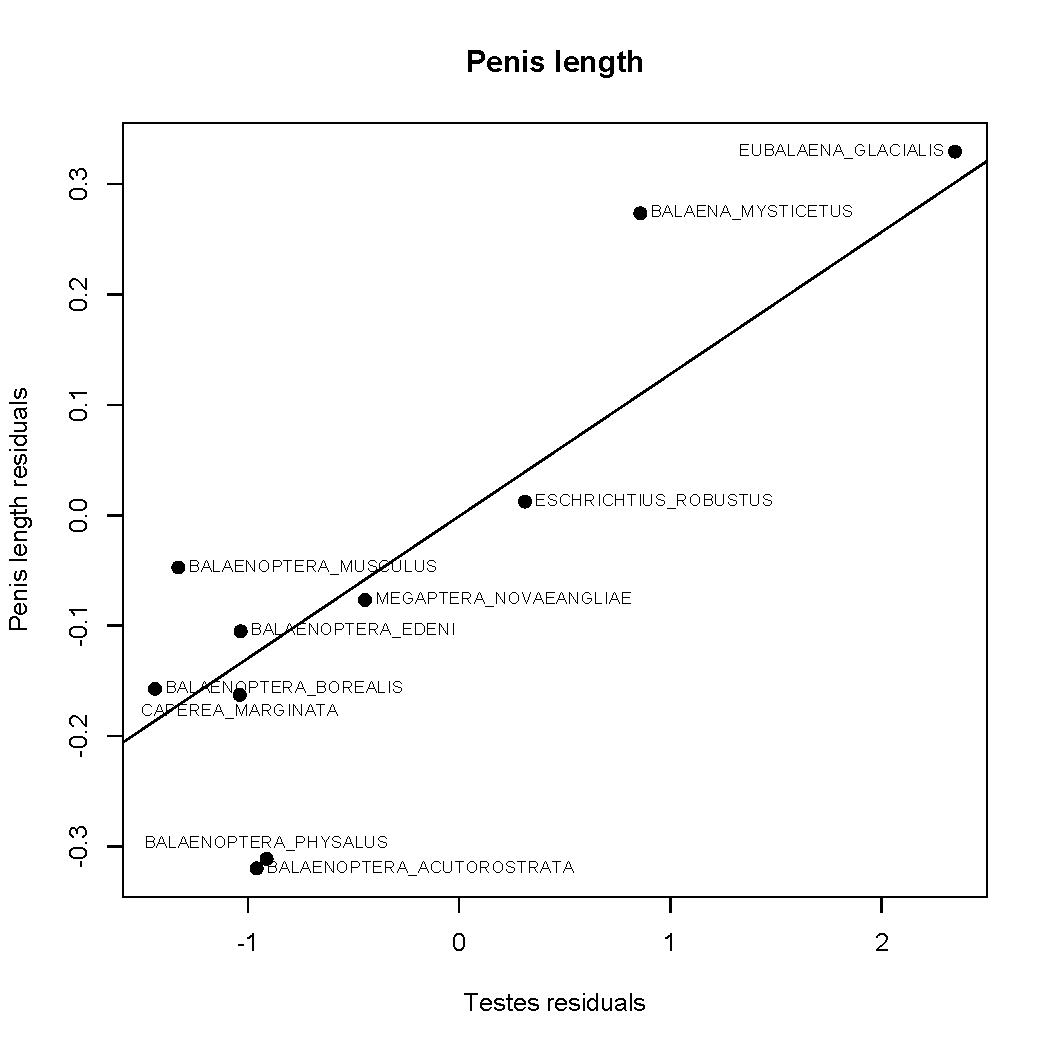
\includegraphics[width=\textwidth]{S1}
\end{center}
\caption{
\textbf{Whale species with relatively large testes have relatively long penises.} 
Two separate regression, each drawn using the GLS procedure in the R package NLME and a correlation structure accounting for phylogenetic relatedness \citep{pagel1999} using the corPagel procedure in the R package APE \citep{paradis2004}, were drawn to derive the residuals of penis length onto body mass, and testes mass onto body mass. A third phylogenetic regression (pictured here) was used to test the correlation of residual penis length with residual testis mass. Raw data taken from Table 2 of \citep{brownell1986}, and analyzed in the phylogenetic framework of \citep{mcgowen2009}
}
\end{figure}


% \begin{landscape}

\begin{figure}
\begin{center}
  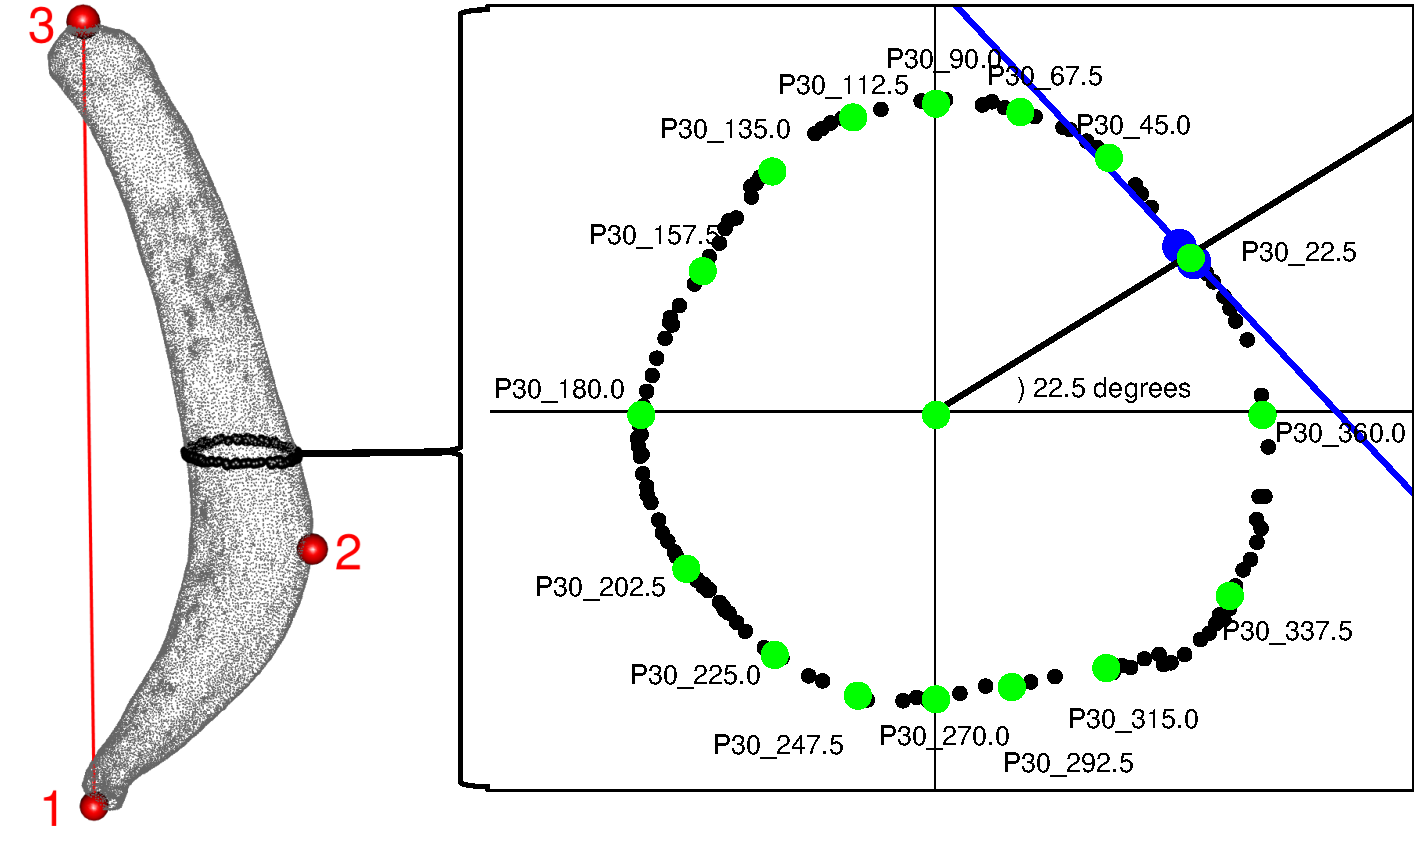
\includegraphics[width=\textwidth]{S2}
\end{center}
\caption{
A series of tools in computational geometry were deployed to define landmarks from pelvic bone scans.  First, the two furthest points apart were found to represent the most posterior and most anterior points (point 1 and 3).  The entire point cloud was transformed so that point 1 was x=0, y=0, z=0, and point 3 was x=0, y=0, with some positive value of z.  A new z-axis was drawn between point 1 and 3 (red line), and the point furthest from this point found (point 2), and the entire point cloud transformed so that point 2 was x=some positive value, y=0, z=some positive value.  After this initial transformation, we sampled points that fell within the most posterior 0.5\% of the z axis, the most anterior 0.5\% of the z axis, or the middle 0.5\% of the z axis (typically, several hundred points sampled each region), and calculated the centroid of their respective convex hulls.  This second transformation accounted for variation in the placement of the first three points.  Then, 60 evenly-spaced slices of points were sampled along the z axis, where each slice thickness was 0.5\% the length of the z-axis.  One slice appears in the right panel as an example.  For each slice, the midpoint of the convex hull was calculated (green point in middle of right panel).  Then, moving in increments of 22.5 degrees from the x-axis (only the first increment shown in detail), we determined the two points straddling the line extending from the centroid (two points shown in blue, one slightly obscured, with connecting line drawn in blue).  A landmark was defined as the intersection of the black and blue lines (green point) and named according to its slice (i.e., P30) and its angle from the x-axis (i.e., 22.5).  Only P30\_22.5 is shown in detail: the other green points are shown for completeness.  All green points correspond to the green points shown in Fig. 1C of the manuscript.  Only the green points were included in downstream analyses; all other points were discarded.
}
\end{figure}
% \end{landscape}

 
% \begin{landscape}
\begin{figure}
\begin{center}
  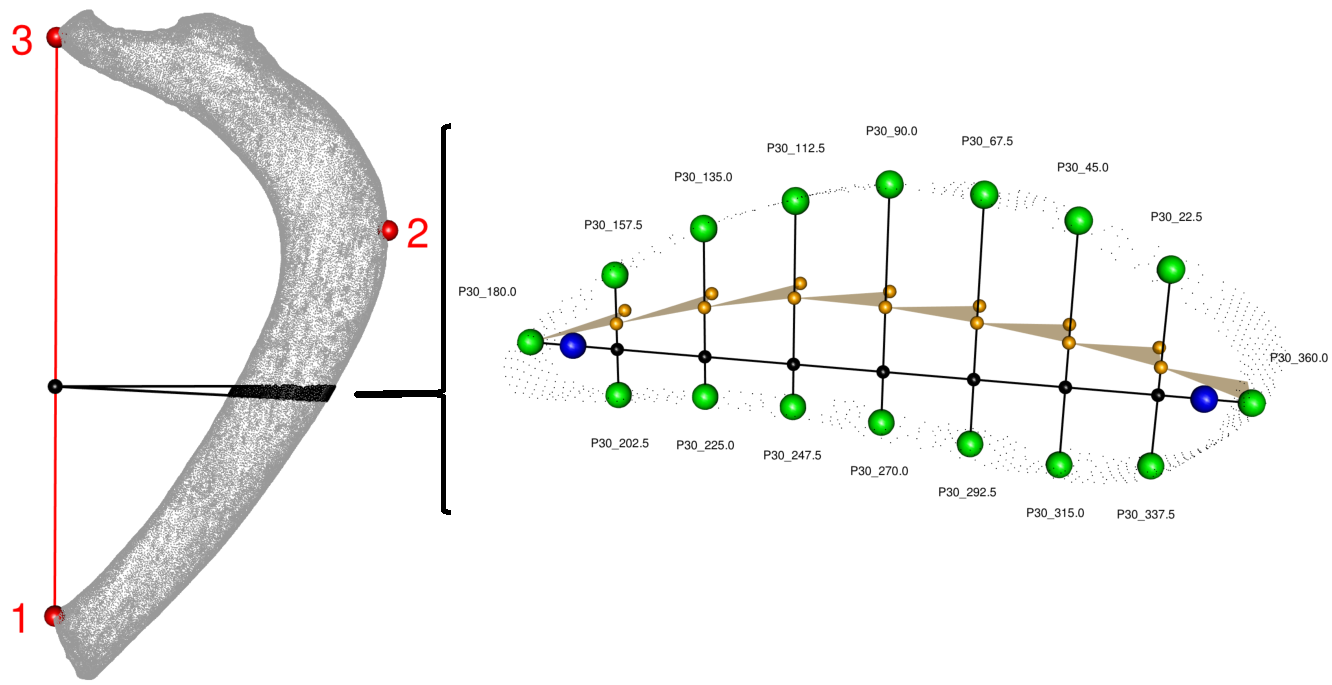
\includegraphics[width=\textwidth]{S3}
\end{center}
\caption{
A series of tools in computational geometry were deployed to define landmarks from rib bone scans.  First, all points were initially transformed according to the same three initial points described above for pelvic bones.  Then, a fulcrum (black sphere) was placed 1/3 up the length of the z-axis, and the bone scan divided into 60 slices of equal angle from that fulcrum.  For each slice (the 30th slice shown as an example in right panel), the centroid of the convex hull of the 20\% most medial points (leftmost blue sphere) and 20\% most lateral points (rightmost blue sphere) points was used to draw a line.  We identified the point on that line which was closest to a point in the original scan (rightmost/leftmost green spheres, right panel).  This line was then divided evenly (black spheres) and lines perpendicular to the black spheres computed.  All points from the original scan within a certain distance to the perpendicular lines were found, projected onto the perpendicular line and the midpoint computed (orange spheres on perpendicular lines, right panel).  The orange sphere was projected onto the plane parallel to the figure to find a third point with which to draw a plane (indicated by orange triangles, right panel).  Those orange triangles allowed us to divide the bone into anterior and posterior halves and to account for complex curvatures.  The corresponding green spheres on the perpendicular lines were determined as done for the medial and lateral green spheres.  All green spheres are named as described in Fig. S2, and correspond to the green spheres shown in Fig. 1D of the manuscript.  Only the green spheres were included in downstream analyses; all other points were discarded. 
}
\end{figure}
% \end{landscape}

 
\begin{figure}
\begin{center}
  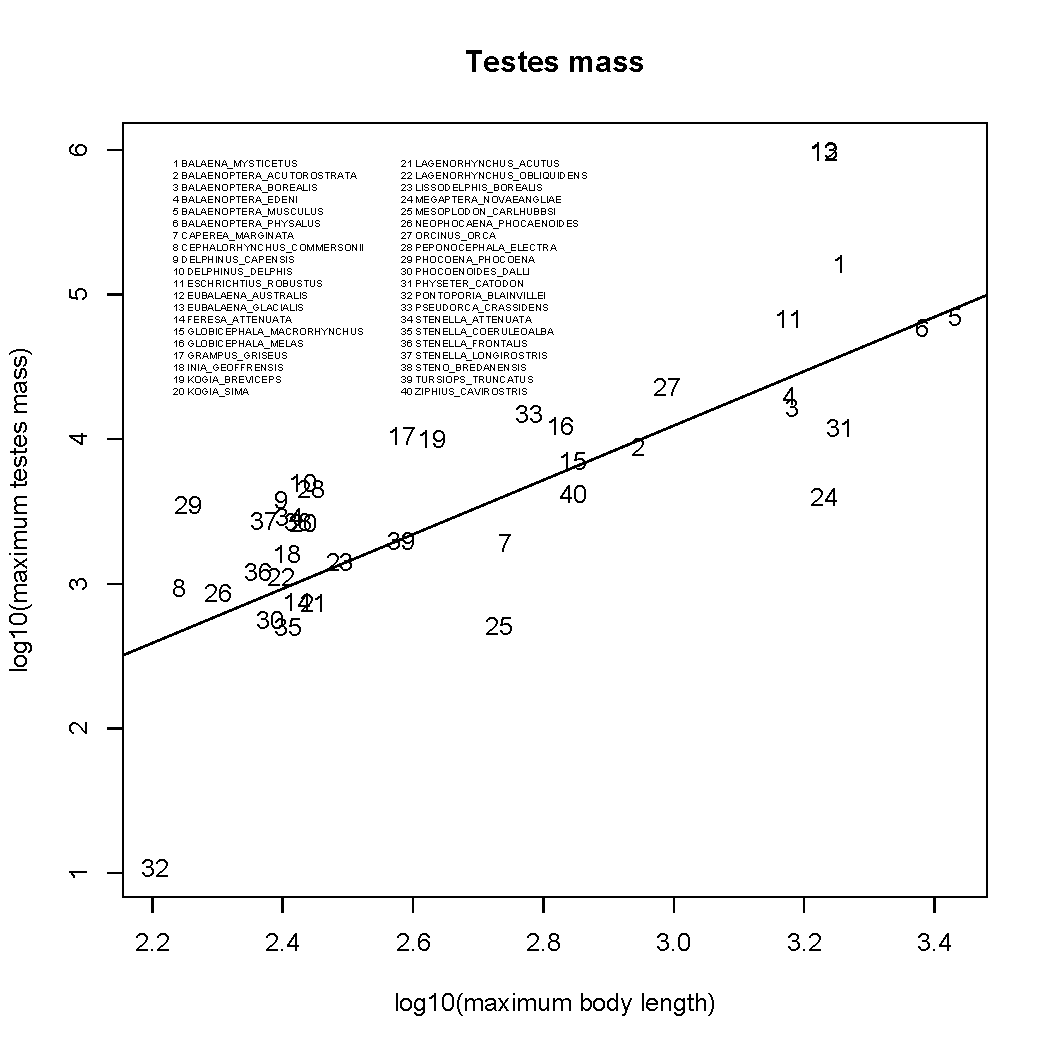
\includegraphics[width=\textwidth]{S4}
\end{center}
\caption{
\textbf{The regression of maximal recorded testis size onto maximal recorded body mass.} 
The regression was drawn using the GLS procedure in the R package NLME,
with a correlation structure that accounted for phylogenetic relatedness \citep{pagel1999}, using the corPagel
procedure in the R package APE \citep{paradis2004}. The phylogenetic residuals were used as a measure of relative
testes size.
}
\end{figure}

\begin{figure}
\begin{center}
  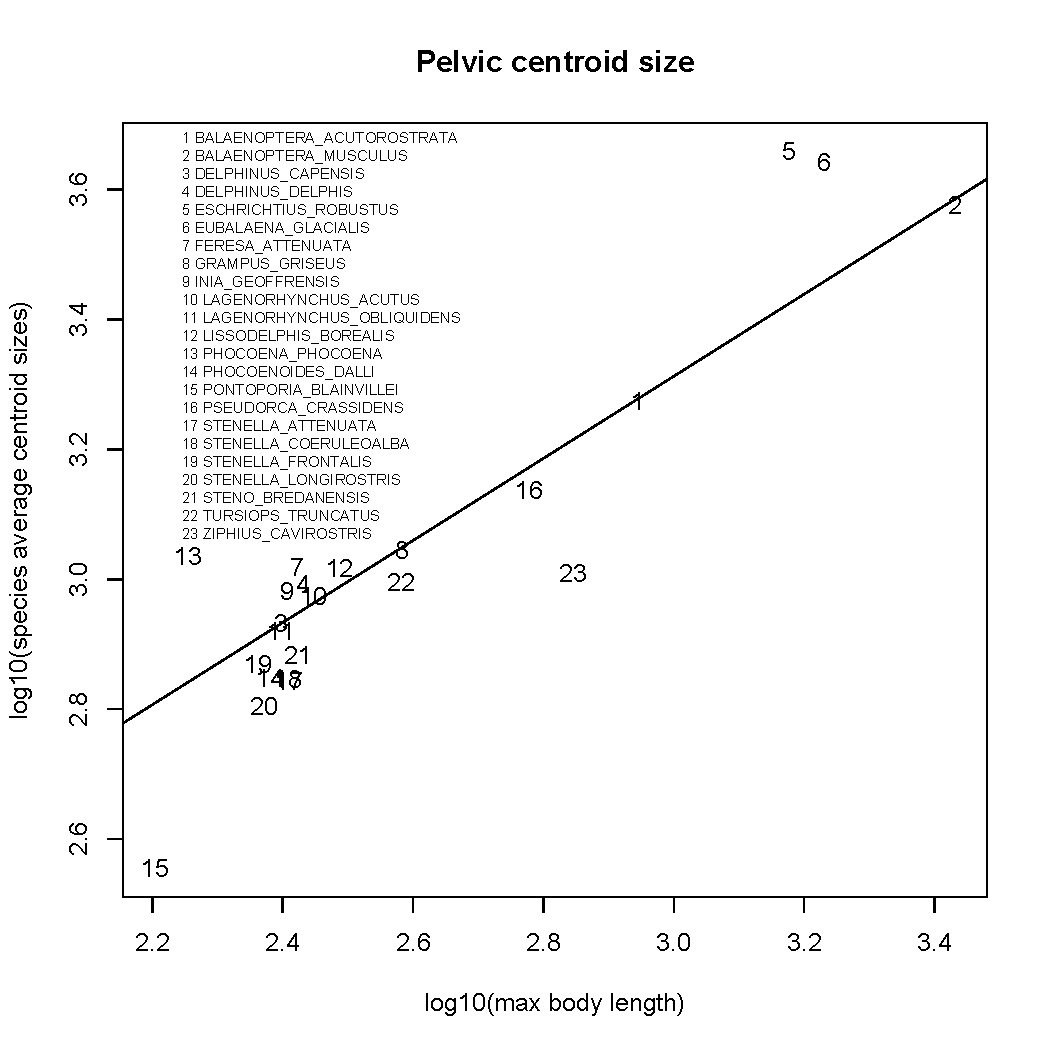
\includegraphics[width=\textwidth]{S5}
\end{center}
\caption{
\textbf{Centroid size onto max body length.} 
For each species (sexually mature males only), an average centroid size was calculated, then regressed onto body length using the gls procedure in the R package nlme, with a correlation structure that accounted for phylogenetic relatedness \citep{pagel1999}, using the corPagel procedure in the R package ape \citep{paradis2004}.  The phylogenetic residuals of centroid size were correlated with the phylogenetic residuals of testis size (supplementary Fig. S6). 
}
\end{figure}

\begin{figure}
\begin{center}
  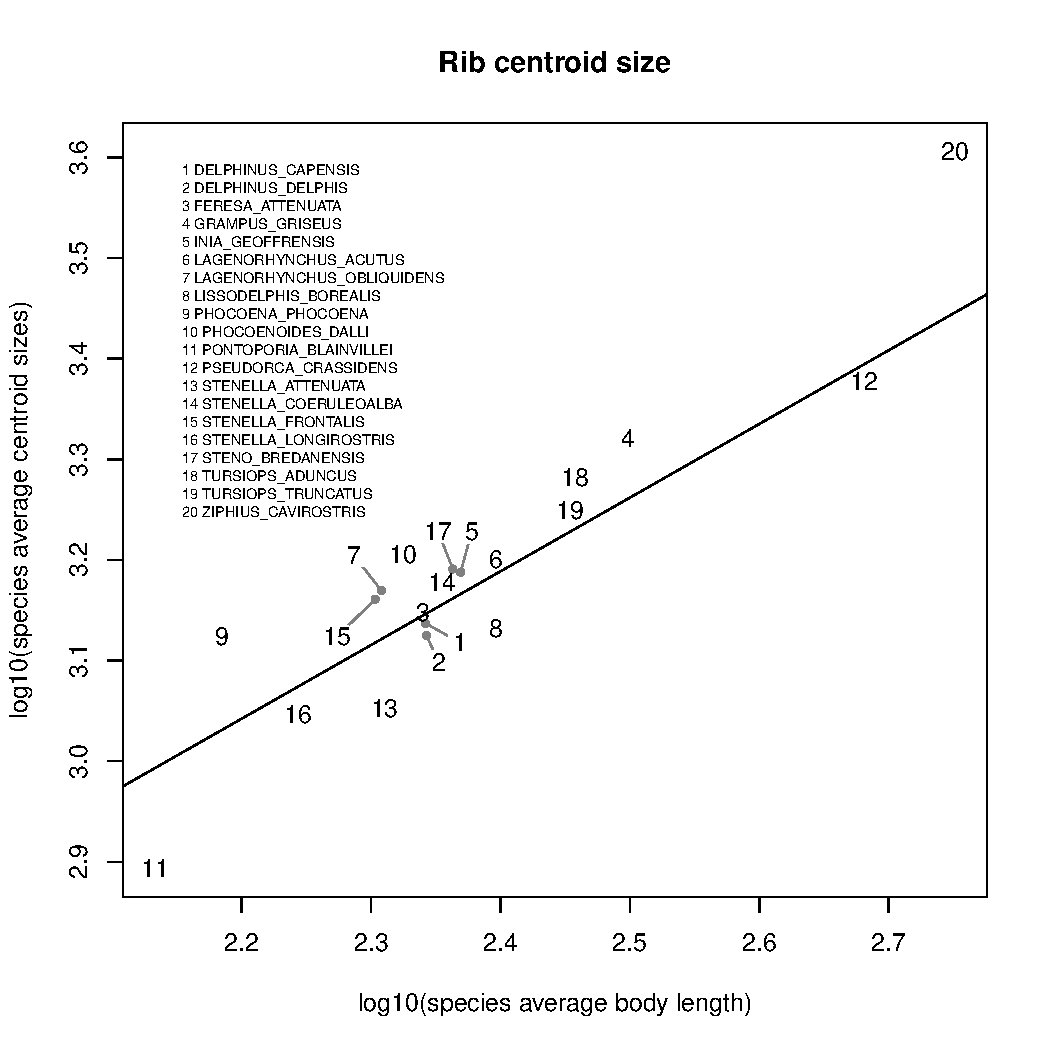
\includegraphics[width=\textwidth]{S6}
\end{center}
\caption{
\textbf{The residuals of centroid size were positively correlated with the
residuals of testis size.}
The regression between testis mass residuals (taken from Fig. S4) and centroid size residuals (taken from Fig. S5) was assessed using the gls procedure in the R package nlme, with a correlation structure that accounts for phylogenetic relatedness \citep{pagel1999}, using the corPagel procedure in the R package ape \citep{paradis2004}.  Centroid size residuals were significantly positively correlated with testis mass residuals (p=0.0012).  Such analyses are standard but do not account for intraspecific variation.  In the main text, we built a customized phylogenetic model in order to account for intraspecific variation.
}
\end{figure}

% 
% \begin{figure}
% \begin{center}
%   \includegraphics[width=\textwidth]{S7}
% \end{center}
% \caption{
% \textbf{As observed for males (Figure 3 of manuscript), the marginal posterior
% distributions of correlations between changes in female pelvic bone size was significantly
% correlated with shifts towards larger testis size.} Under a phylogenetic model of correlated trait
% evolution (supplementary methods), the size of the pelvic bone is positively correlated with shifts
% towards larger testes after accounting for body size evolution (red), while rib bone size does not show
% this correlation (gray). Only sexually mature females were included in this analysis.
% }
% \end{figure}

\begin{figure}[ht]
  \begin{center}
    \includegraphics{../males/posterior-correlations}
  \end{center}
  \caption{\textbf{Marginal posterior distributions of correlations}, 
  with length fixed, between changes in rib size, pelvic bone size, and testes size.
  Rib-testes and pelvis-testes correlations were also displayed in figure 3 of the manuscript.
  \label{fig:males_posterior_cors}
  }
\end{figure}

\begin{figure}[ht]
  \begin{center}
    \includegraphics{../males-complete/posterior-correlations}
  \end{center}
  \caption{
  \textbf{The marginal posterior distributions of correlation coefficients} 
  do not change when restricting to bones from adult male cetaceans for which we have both data for both ribs and pelvic bones,
  which excludes baleen whales.  (compare to figure \ref{fig:males_posterior_cors}).
  \label{fig:males_complete_posterior_cors}
  }
\end{figure}

\begin{figure}[ht]
  \begin{center}
    \includegraphics{../females/posterior-correlations}
  \end{center}
  \caption{
  \textbf{As observed for males (Figure \ref{fig:males_posterior_cors} and figure 3 of manuscript), the marginal posterior
distributions of correlations between changes in female pelvic bone size was significantly
correlated with shifts towards larger testis size.} Under a phylogenetic model of correlated trait
evolution (supplementary methods), the size of the pelvic bone is positively correlated with shifts
towards larger testes after accounting for body size evolution (red), while rib bone size does not show
this correlation (gray). Only sexually mature females were included in this analysis.
  between changes in rib size, pelvic bone size, and testes size.
  \label{fig:female_posterior_cors}
  }
\end{figure}



\processdelayedfloats

\bibliography{correlated-traits}

\end{document}
